\documentclass{article}
\usepackage{float, hyperref}
\usepackage[margin=1in]{geometry}
\usepackage{graphicx}
\usepackage{hyperref}
\usepackage{caption}

\usepackage{Sweave}
\begin{document}
\Sconcordance{concordance:Significance.tex:Significance.Rnw:%
1 7 1 1 0 7 1 1 5 2 1 1 19 1 8 2 1 1 2 5 0 1 2 3 1 1 2 1 0 1 1 3 0 1 2 %
9 1 1 3 5 0 1 2 2 1 1 2 5 0 1 2 3 1 1 3 2 0 1 1 4 0 1 3 2 1 1 2 5 0 1 2 %
5 1 1 2 5 0 1 2 3 1 1 4 3 0 1 3 1 0 1 1 11 0 1 3 1 0 1 1 1 2 36 0 1 2 2 %
1 1 2 1 0 1 1 4 0 1 2 3 1 1 3 5 0 1 2 1 4 3 0 1 4 3 0 1 8 6 0 2 1 1 4 2 %
0 1 2 3 1 1 3 1 0 1 2 1 0 1 2 1 0 1 2 1 0 1 2 1 0 2 2 1 0 1 2 5 1 1 2 1 %
0 1 2 1 0 2 1 3 0 1 2 2 1 1 2 5 0 1 2 5 1 1 2 1 0 1 1 4 0 1 2 3 1 1 5 4 %
0 3 1 1 5 3 0 1 8 6 0 2 1 1 4 2 0 1 2 3 1 1 3 1 0 1 2 1 0 1 2 1 0 1 2 1 %
0 1 2 1 0 2 2 1 0 1 2 5 1 1 2 1 0 1 2 1 0 2 1 3 0 1 2 2 1 1 2 5 0 1 2 5 %
1 1 2 1 0 1 1 4 0 1 2 3 1 1 3 2 0 1 1 1 19 21 0 1 2 1 3 2 0 1 2 1 0 1 2 %
4 0 1 2 2 1 1 2 5 0 1 2 3 1 1 4 3 0 1 1 3 0 1 2 2 1 1 2 5 0 1 2 5 1 1 2 %
5 0 1 2 3 1 1 30 32 0 1 2 1 1}


\author{Lindsay Rutter}
\title{Cluster Analysis of Wasps}

\maketitle

  
\section*{Introduction}



\begin{figure}[H]
\centering
\begin{Schunk}
\begin{Sinput}
> ggparcoord(data.frame(d[[1]]), columns=1:30, alphaLines=0, boxplot=TRUE, scale="globalminmax") + coord_flip()
\end{Sinput}
\end{Schunk}
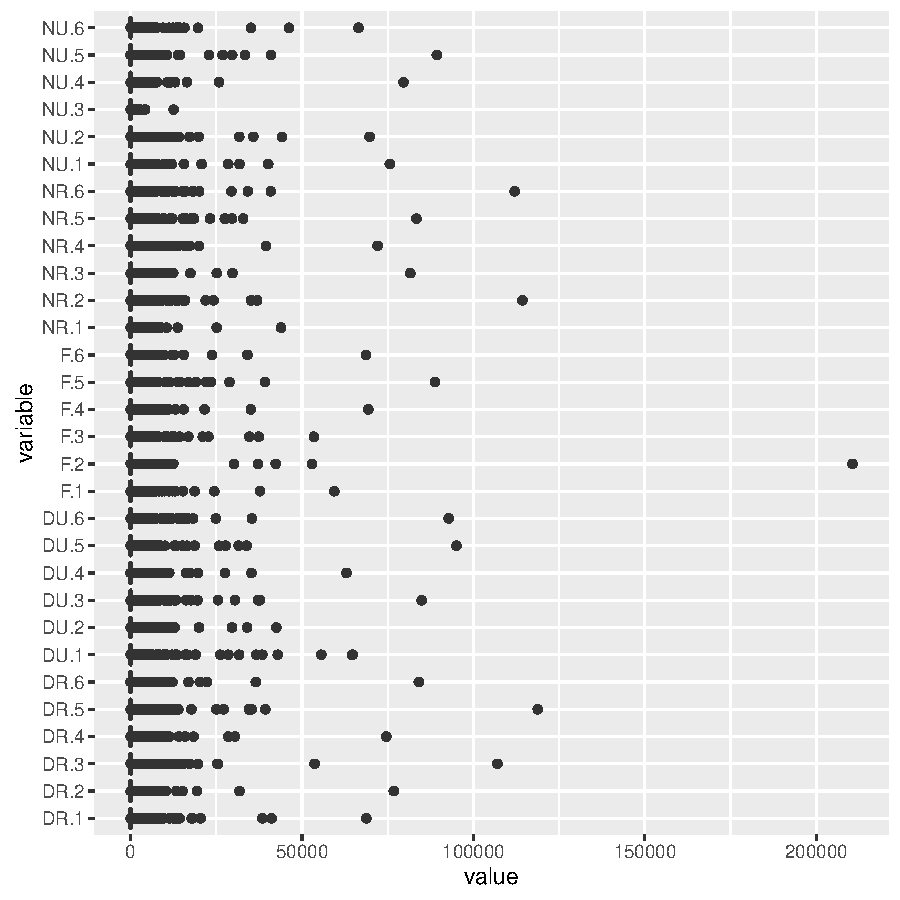
\includegraphics{Significance-004}
\caption{Boxplot of all samples.}
\label{BoxAll}
\end{figure}

\begin{Schunk}
\begin{Sinput}
> myVec = c("DR", "DU", "F", "NR", "NU")
> myCol = c(which(colnames(countTable) == grep('DR', colnames(countTable), value=TRUE)), which(colnames(countTable) == grep('DU', colnames(countTable), value=TRUE)))
\end{Sinput}
\end{Schunk}

%\begin{figure}[H]
%\centering
%<<fig=TRUE, echo=TRUE>>=
%scatmat(countTable, columns=myCol, alpha = 0.01)
%@
%\caption{Scatterplot matrix of DU and DR.}
%\label{BoxAll}
%\end{figure}

\begin{Schunk}
\begin{Sinput}
> # estimate normalization factors
> d = calcNormFactors(d)
\end{Sinput}
\end{Schunk}

\begin{figure}[H]
\centering
\begin{Schunk}
\begin{Sinput}
> plotMDS(d, labels=colnames(countTable), col = c("red","orange","green","blue","purple")[factor(listcond)])
\end{Sinput}
\end{Schunk}
\includegraphics{Significance-007}
\caption{MDS of all samples. NU.3 looks very poor. F.2 does as well. Possibly NU.4 is poor.}
\label{plotMDS}
\end{figure}

\begin{Schunk}
\begin{Sinput}
> # estimate tagwise dispersion
> d = estimateCommonDisp(d)
> d = estimateTagwiseDisp(d)
> # Now, str(d) has raw read counts, norm factors, lib.size, and more
\end{Sinput}
\end{Schunk}

\begin{figure}[H]
\centering
\begin{Schunk}
\begin{Sinput}
> plotMeanVar(d, show.tagwise.vars=TRUE, NBline=TRUE)
\end{Sinput}
\end{Schunk}
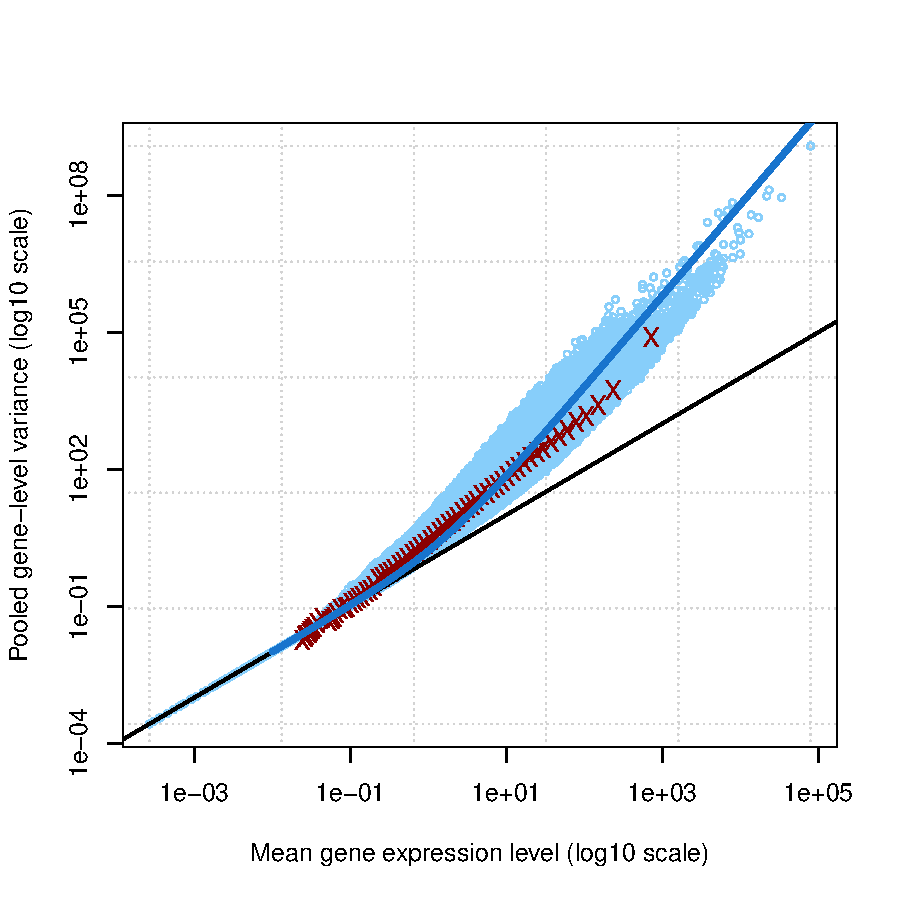
\includegraphics{Significance-009}
\caption{This function is useful for exploring the mean-variance relationship in the data. Raw variances are, for each gene, the pooled variance of the counts from each sample, divided by a scaling factor (by default the effective library size). The function will plot the average raw variance for genes split into nbins bins by overall expression level. The averages are taken on the square-root scale as for count data the arithmetic mean is upwardly biased. A line showing the Poisson mean-variance relationship (mean equals variance) is always shown.}
\label{plotMeanVar}
\end{figure}

\begin{figure}[H]
\centering
\begin{Schunk}
\begin{Sinput}
> plotBCV(d)
\end{Sinput}
\end{Schunk}
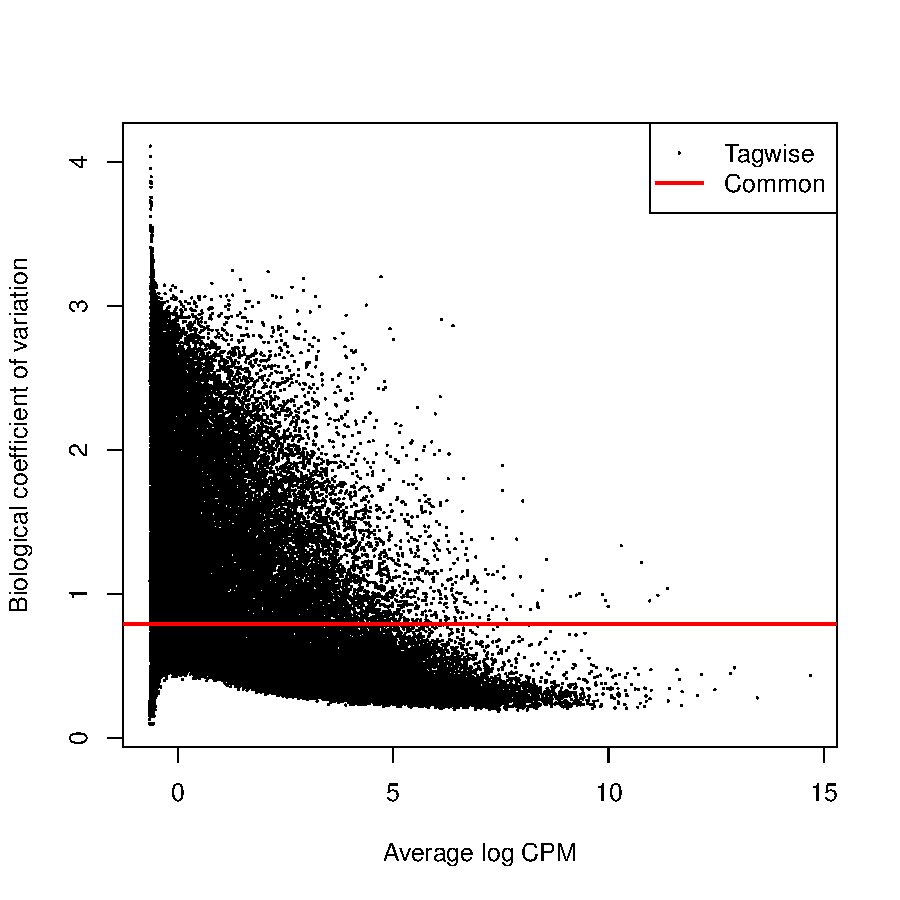
\includegraphics{Significance-010}
\caption{Plots the tagwise biological coefficient of variation (square root of dispersions) against log2-CPM.}
\label{plotBCV}
\end{figure}

\begin{Schunk}
\begin{Sinput}
> # Test for differential expression
> # Compute genewise exact tests for differences in the means between two groups of negative-binomially distributed counts. The functions accept two groups of count libraries, and a test is performed for each row of data. For each row, the test is conditional on the sum of counts for that row. No genes passed FDR correction
> de = exactTest(d, pair=c("NU","DR"))
> #Use the topTags function to present a tabular summary of the differential expression statistics (note that topTags operates on the output of exactTest. This automatically sorts by ascending p-value, and creates an FDR column (by dividing p-value by the number of genes)
> tt = topTags(de, n=nrow(d))
> head(tt$table)
\end{Sinput}
\begin{Soutput}
          logFC    logCPM       PValue       FDR
34808  6.068273 1.3124579 1.791310e-06 0.2824735
89828  6.155402 0.2691713 7.118592e-06 0.5612689
38343 -9.117725 2.5869741 1.211436e-05 0.6367751
79792  7.738891 4.0912902 1.885500e-05 0.7079621
84117  2.056710 3.6192123 2.244776e-05 0.7079621
81034  7.833797 2.8494281 2.811878e-05 0.7390131
\end{Soutput}
\begin{Sinput}
> # Inspect the depth-adjusted reads per million for some of the top differentially expressed genes (just dividing each read count by 1/millionth lib.size)
> nc = cpm(d, normalized.lib.sizes=TRUE)
> rn = rownames(tt$table)
> # Sorted in order of lowest FDR from DE comparison
> head(nc[rn,order(listcond)],5)
\end{Sinput}
\begin{Soutput}
           DR.1     DR.2      DR.3      DR.4      DR.5      DR.6      DU.1
34808  2.792674  0.00000  0.000000  5.683925  2.207572  5.265151  1.710986
89828  1.787735  0.00000  3.312755  4.646608  4.305916  2.772979  0.000000
38343  0.000000  0.00000  0.113717  0.000000  0.000000  0.000000  0.000000
79792 12.215306  0.00000  0.000000  0.000000 38.353693  0.000000 48.154032
84117 16.935878 12.97072 22.958857 15.989591  9.229837 14.005301 19.554525
           DU.2      DU.3      DU.4      DU.5      DU.6         F.1         F.2
34808  1.237378  4.686304  1.361842  2.530349  1.999975 2.014017350 0.000000000
89828  0.000000  0.000000  0.000000  0.000000  0.000000 0.000000000 0.000000000
38343  0.000000  0.000000  0.000000  0.000000  0.000000 0.003151827 0.004250863
79792 24.792177 10.810026 35.374421 36.808222 31.779262 5.767843116 4.314625580
84117  8.831191  7.545109  5.132838 16.609549 17.599779 8.065524882 6.648349169
            F.3      F.4          F.5      F.6      NR.1      NR.2      NR.3
34808  1.425218  0.00000  3.222709369  1.10184  2.273195  3.808794  1.608547
89828  0.000000  0.00000  0.000000000  0.00000  0.000000  0.000000  0.000000
38343  0.000000  0.00000  0.002768651  0.00000  0.000000  0.000000  0.000000
79792 23.730171  0.00000 38.423333864 20.29847 32.315742 39.607136 47.310773
84117 18.287364 16.86495 21.116498586 11.23156  5.669349  8.577221 17.609525
           NR.4      NR.5        NR.6      NU.1     NU.2     NU.3      NU.4
34808  4.111939  2.392347  3.14834177 0.0000000 0.000000   0.0000  0.000000
89828  0.000000  0.000000  0.00000000 0.0000000 0.000000   0.0000  0.000000
38343  0.000000  0.000000  0.02672616 0.0000000 0.000000 118.5125 28.766266
79792 23.917779  0.000000 15.80050642 0.0000000 0.000000   0.0000  0.000000
84117 17.424342 17.139455 11.41741600 0.8991105 1.857902   0.0000  6.792142
          NU.5      NU.6
34808 0.000000  0.000000
89828 0.000000  0.000000
38343 0.000000 49.821681
79792 0.000000  0.000000
84117 4.286813  6.072133
\end{Soutput}
\end{Schunk}

\begin{figure}[H]
\centering
\begin{Schunk}
\begin{Sinput}
> deg = rn[tt$table$FDR < .05]
> plotSmear(d, de.tags=deg)
\end{Sinput}
\end{Schunk}
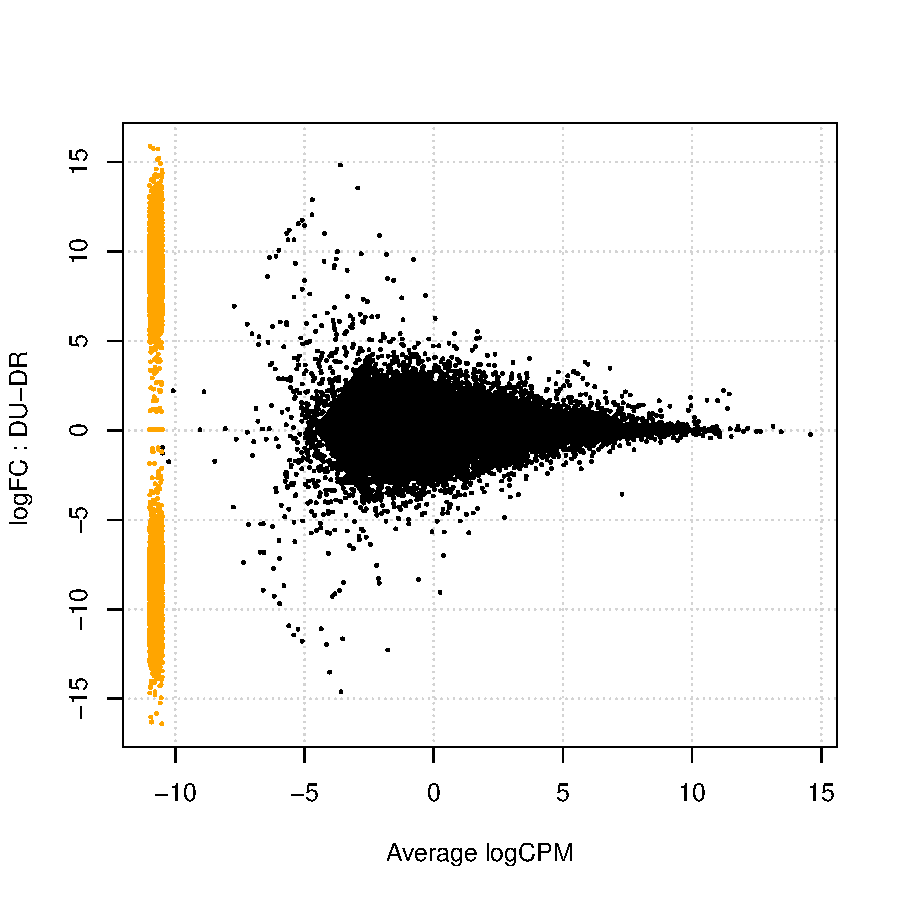
\includegraphics{Significance-012}
\caption{Create a graphical summary, such as an M (log-fold change) versus A (log-average expression) plot, here showing the genes selected as differentially expressed with a 5\% false discovery rate. There were none in this dataset!}
\label{plotSmear}
\end{figure}

\begin{Schunk}
\begin{Sinput}
> # Would save file
> write.csv(tt$table, file="toptags_edgeR.csv")
\end{Sinput}
\end{Schunk}

\begin{Schunk}
\begin{Sinput}
> ########## Is there any step in the edgeR package where genes are eliminated for low mean and/or stdev read counts? ##########
> 
> d2 <- DGEList(counts=countTable)
> # 38,280 genes (from 157,691).
> #d2 <- d2[rowSums(d2$counts>1)>=ncol(d2)/2,]
> # 52,564 genes (from 157,691). In edgeR, it is recommended to remove features without at least 1 read per million in n of the samples, where n is the size of the smallest group of replicates. Also, should filter on CPM!
> d2 <- d2[rowSums(d2$counts>1)>=6,]
> # Took too long as well
> #d2plot = as.data.frame(d2[[1]])
> #d2plot = gather(d2plot)
> #ggplot(d2plot, aes(factor(value), key)) + geom_boxplot()
> 
> # Now positive and negative
> cpm.d2.new <- cpm(d2, TRUE, TRUE)
> cpm.d2.norm <- betweenLaneNormalization(cpm.d2.new, which="full", round=FALSE)
> d2 = cpm.d2.norm
> RowSD = function(x) {
+   sqrt(rowSums((x - rowMeans(x))^2)/(dim(x)[2] - 1))
+ }
> d2t = d2
> d2 = as.data.frame(d2t)
> d2 = mutate(d2, mean = (DR.1+DR.2+DR.3+DR.4+DR.5+DR.6+DU.1+DU.2+DU.3+DU.4+DU.5+DU.6+F.1+F.2+F.3+F.4+F.5+F.6+NR.1+NR.2+NR.3+NR.4+NR.5+NR.6+NU.1+NU.2+NU.3+NU.4+NU.5+NU.6)/ncol(d2), stdev = RowSD(cbind(DR.1,DR.2,DR.3,DR.4,DR.5,DR.6,DU.1,DU.2,DU.3,DU.4,DU.5,DU.6,F.1,F.2,F.3,F.4,F.5,F.6,NR.1,NR.2,NR.3,NR.4,NR.5,NR.6,NU.1,NU.2,NU.3,NU.4,NU.5,NU.6)))
> rownames(d2)=rownames(d2t)
> # The first quartile threshold of mean counts across the 5 samples
> q1T = as.numeric(summary(d2$mean)["1st Qu."])
> # (39,427, 31)
> d2q1 = subset(d2,mean>q1T)
> # The first quartile threshold of standard deviation across the 5 samples
> q1Ts = as.numeric(summary(d2q1$stdev)["1st Qu."])
> # L120q1 (29572, 31)
> d2q1 = subset(d2q1,stdev>q1Ts)
> # filt (22992, 31)
> filt = subset(d2,mean<=q1T|stdev<=q1Ts)
> model = loess(mean ~ stdev, data=d2q1)
> # (11855, 32)
> d2q1 = d2q1[which(sign(model$residuals) == 1),]
> d2q1 = d2q1[,1:(ncol(d2q1)-2)]
> d2q1s = t(apply(as.matrix(d2q1), 1, scale))
> colnames(d2q1s)=colnames(d2q1)
> colnames(d2q1)=colnames(d2q1) 
> filt = filt[,1:(ncol(filt)-2)]
> colnames(filt)=colnames(d2q1)
> # filt (40709, 32)
> filt = rbind(filt,d2q1[which(sign(model$residuals) == -1),])
> # filt (40709, 32)
> filts = t(apply(as.matrix(filt), 1, scale))
> colnames(filts)=colnames(d2q1)
> colnames(filt)=colnames(d2q1)
\end{Sinput}
\end{Schunk}

\begin{figure}[H]
\centering
\begin{Schunk}
\begin{Sinput}
> ggparcoord(d2q1, columns=1:ncol(d2q1), alphaLines=0, boxplot=TRUE, scale="globalminmax") + coord_flip() + scale_y_log10()
\end{Sinput}
\end{Schunk}
\includegraphics{Significance-015}
\caption{This is d2q1. Looks better than d2q1s.png (only strange one is NU.3)}
\label{Boxd2q1}
\end{figure}

\begin{figure}[H]
\centering
\begin{Schunk}
\begin{Sinput}
> d2q1s_Plot = as.data.frame(d2q1s)
> ggparcoord(d2q1s_Plot, columns=1:ncol(d2q1s_Plot), alphaLines=0, boxplot=TRUE, scale="globalminmax") + scale_y_log10() + coord_flip()
\end{Sinput}
\end{Schunk}
\includegraphics{Significance-016}
\caption{This is d2q1s. Does not look as good as d2q1.png (strange ones are NU.3 and F.2)}
\label{Boxd2q1s}
\end{figure}

\begin{Schunk}
\begin{Sinput}
> # Removing NU.3 and starting over!
> ######################################################################
> 
> rm(list=ls())
> load("All_wasp.rda")
> countTable = select(countTable,-NU.3)
> d2 <- DGEList(counts=countTable)
> # 38,280 genes (from 157,691).
> #d2 <- d2[rowSums(d2$counts>1)>=ncol(d2)/2,]
> # 52,564 genes (from 157,691). In edgeR, it is recommended to remove features without at least 1 read per million in n of the samples, where n is the size of the smallest group of replicates. Should be after CPM
> d2 <- d2[rowSums(d2$counts>1)>=5,]
> # Took too long as well
> #d2plot = as.data.frame(d2[[1]])
> #d2plot = gather(d2plot)
> #ggplot(d2plot, aes(factor(value), key)) + geom_boxplot()
> 
> # Now positive and negative
> cpm.d2.new <- cpm(d2, TRUE, TRUE)
> cpm.d2.norm <- betweenLaneNormalization(cpm.d2.new, which="full", round=FALSE)
> d2 = cpm.d2.norm
> RowSD = function(x) {
+   sqrt(rowSums((x - rowMeans(x))^2)/(dim(x)[2] - 1))
+ }
> d2t = d2
> d2 = as.data.frame(d2)
> d2 = mutate(d2, mean = (DR.1+DR.2+DR.3+DR.4+DR.5+DR.6+DU.1+DU.2+DU.3+DU.4+DU.5+DU.6+F.1+F.2+F.3+F.4+F.5+F.6+NR.1+NR.2+NR.3+NR.4+NR.5+NR.6+NU.1+NU.2+NU.4+NU.5+NU.6)/ncol(d2), stdev = RowSD(cbind(DR.1,DR.2,DR.3,DR.4,DR.5,DR.6,DU.1,DU.2,DU.3,DU.4,DU.5,DU.6,F.1,F.2,F.3,F.4,F.5,F.6,NR.1,NR.2,NR.3,NR.4,NR.5,NR.6,NU.1,NU.2,NU.4,NU.5,NU.6)))
> rownames(d2)=rownames(d2t)
> # The first quartile threshold of mean counts across the 5 samples
> q1T = as.numeric(summary(d2$mean)["1st Qu."])
> # (41202, 31)
> d2q1 = subset(d2,mean>q1T)
> # The first quartile threshold of standard deviation across the 5 samples
> q1Ts = as.numeric(summary(d2q1$stdev)["1st Qu."])
> # L120q1 (30901, 31)
> d2q1 = subset(d2q1,stdev>q1Ts)
> # filt (24031, 31)
> filt = subset(d2,mean<=q1T|stdev<=q1Ts)
> model = loess(mean ~ stdev, data=d2q1)
> # (12262, 31)
> d2q1 = d2q1[which(sign(model$residuals) == 1),]
> d2q1 = d2q1[,1:(ncol(d2q1)-2)]
> d2q1s = t(apply(as.matrix(d2q1), 1, scale))
> colnames(d2q1s)=colnames(d2q1)
> colnames(d2q1)=colnames(d2q1) 
> filt = filt[,1:(ncol(filt)-2)]
> colnames(filt)=colnames(d2q1)
> # filt (42670, 29)
> filt = rbind(filt,d2q1[which(sign(model$residuals) == -1),])
> # filts (42670, 29)
> filts = t(apply(as.matrix(filt), 1, scale))
> colnames(filts)=colnames(d2q1)
> colnames(filt)=colnames(d2q1)
\end{Sinput}
\end{Schunk}

\begin{figure}[H]
\centering
\begin{Schunk}
\begin{Sinput}
> ggparcoord(d2q1, columns=1:ncol(d2q1), alphaLines=0, boxplot=TRUE, scale="globalminmax") + coord_flip() + scale_y_log10()
\end{Sinput}
\end{Schunk}
\includegraphics{Significance-018}
\caption{d2q1 NU.3 removed.}
\label{Boxd2q1NONU3}
\end{figure}

\begin{figure}[H]
\centering
\begin{Schunk}
\begin{Sinput}
> d2q1s_Plot = as.data.frame(d2q1s)
> ggparcoord(d2q1s_Plot, columns=1:ncol(d2q1s_Plot), alphaLines=0, boxplot=TRUE, scale="globalminmax") + scale_y_log10() + coord_flip()
\end{Sinput}
\end{Schunk}
\includegraphics{Significance-019}
\caption{d2q1s NU.3 removed.}
\label{Boxd2q1sNONU3}
\end{figure}

\begin{Schunk}
\begin{Sinput}
> #### Print pairwise scat matrix
> dev.off()
> myVec = c("DR", "DU", "F", "NR", "NU")
> for (i in 1:(length(myVec)-1)){
+   for (j in (i+1):length(myVec)){
+     type1 = myVec[i]
+     type2 = myVec[j]
+     myCol = c(grep(type1, colnames(d2q1)), grep(type2, colnames(d2q1)))
+     jpeg(file = paste(getwd(), "/", type1, "_", type2, "_ALPHA10.jpg", sep=""), height = 700, width = 700)
+     print(scatmat(d2q1, columns=myCol, alpha = 0.01))
+     dev.off()
+     jpeg(file = paste(getwd(), "/", type1, "_", type2, "_ALPHA7.jpg", sep=""), height = 700, width = 700)
+     print(scatmat(d2q1, columns=myCol, alpha = 0.007))
+     dev.off()
+     jpeg(file = paste(getwd(), "/", type1, "_", type2, "_ALPHA3.jpg", sep=""), height = 700, width = 700)
+     print(scatmat(d2q1, columns=myCol, alpha = 0.003))
+     dev.off()
+     jpeg(file = paste(getwd(), "/", type1, "_", type2, "_ALPHA1.jpg", sep=""), height = 700, width = 700)
+     print(scatmat(d2q1, columns=myCol, alpha = 0.001))
+     dev.off()    
+     }
+ }
\end{Sinput}
\end{Schunk}

\begin{Schunk}
\begin{Sinput}
> ############ Significance testing for normalized no NU.3 ###########
> listcond = c(rep(c("DR","DU","F","NR"),each=6), rep(c("NU"),each=5))
> # create DGEList object
> d = DGEList(counts=countTable, group=listcond)
> # estimate normalization factors
> d = calcNormFactors(d)
\end{Sinput}
\end{Schunk}

\begin{figure}[H]
\centering
\begin{Schunk}
\begin{Sinput}
> plotMDS(d, labels=colnames(countTable), col = c("red","orange","green","blue","purple")[factor(listcond)])
\end{Sinput}
\end{Schunk}
\includegraphics{Significance-022}
\caption{MDS plot NU.3 removed.}
\label{MDS-NONU3}
\end{figure}

\begin{Schunk}
\begin{Sinput}
> # Estimate tagwise dispersion
> # Now, str(d) has raw read counts, norm factors, lib.size, and more
> d = estimateCommonDisp(d)
> d = estimateTagwiseDisp(d)
\end{Sinput}
\end{Schunk}

\begin{figure}[H]
\centering
\begin{Schunk}
\begin{Sinput}
> plotMeanVar(d, show.tagwise.vars=TRUE, NBline=TRUE)
\end{Sinput}
\end{Schunk}
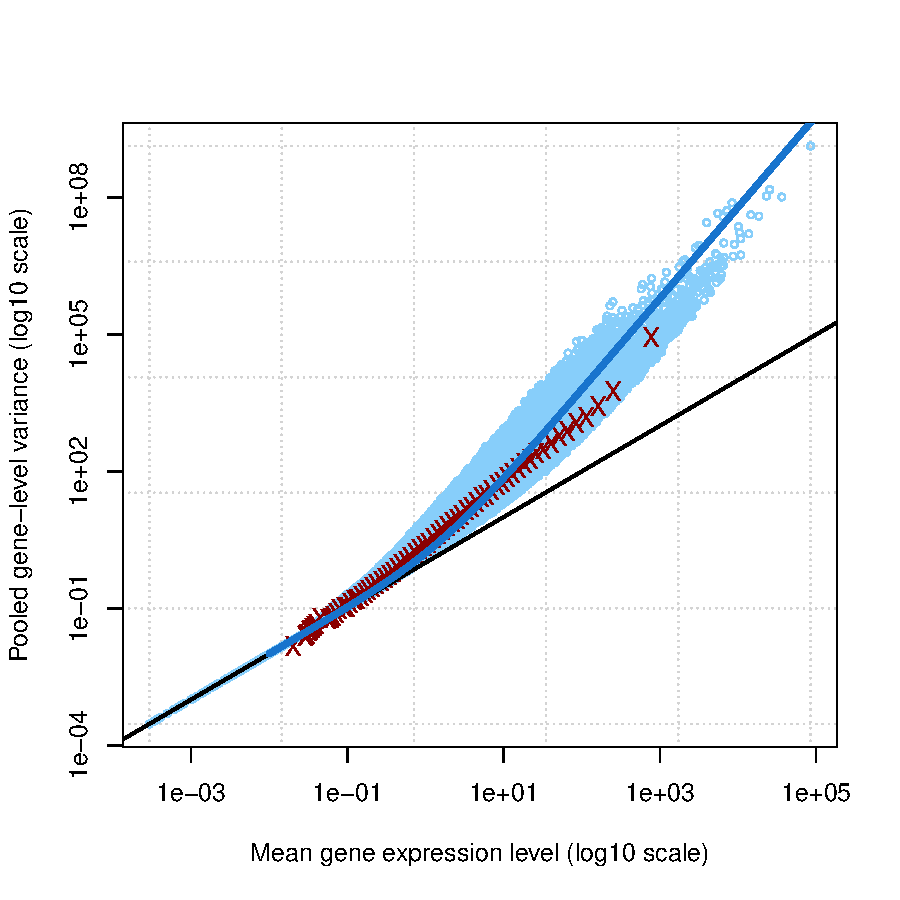
\includegraphics{Significance-024}
\caption{MDS plot NU.3 removed.}
\label{MeanVarPlot-NONU3}
\end{figure}

\begin{figure}[H]
\centering
\begin{Schunk}
\begin{Sinput}
> plotBCV(d)
\end{Sinput}
\end{Schunk}
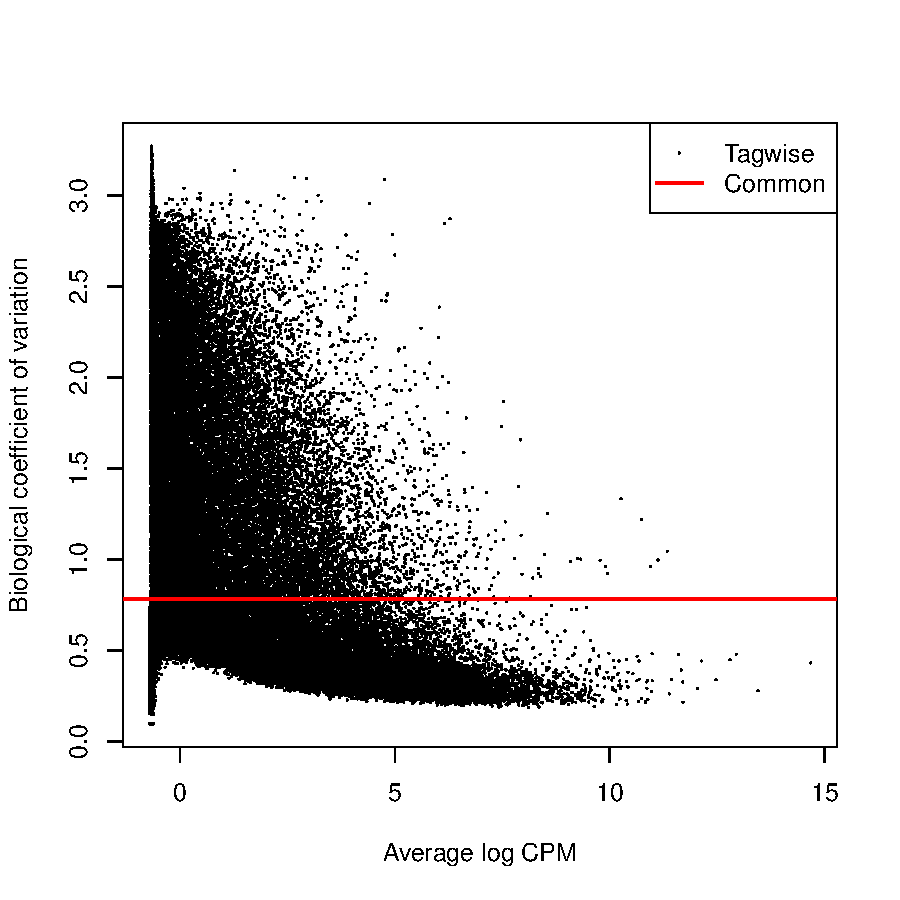
\includegraphics{Significance-025}
\caption{MDS plot NU.3 removed.}
\label{BCV-NONU3}
\end{figure}

\begin{Schunk}
\begin{Sinput}
> ######### Create pairwise significance tests #########
> 
> for (i in 1:(length(myVec)-1)){
+   for (j in (i+1):length(myVec)){
+ 
+   # Test for differential expression
+   de = exactTest(d, pair=c(myVec[i],myVec[j]))
+ 
+   #This automatically sorts by ascending p-value, and creates an FDR column (by dividing p-value by the number of genes)
+   tt = topTags(de, n=nrow(d))
+   head(tt$table)
+ 
+   # Inspect the depth-adjusted reads per million for some of the top differentially expressed genes (just dividing each read count by 1/millionth lib.size)
+   nc = cpm(d, normalized.lib.sizes=TRUE)
+   rn = rownames(tt$table)
+   # Sorted in order of lowest FDR from DE comparison
+   head(nc[rn,order(listcond)],5)
+ 
+   # Create a graphical summary, such as an M (log-fold change) versus A (log-average expression) plot, here showing the genes selected as differentially expressed with a 5% false discovery rate.
+   deg = rn[tt$table$FDR < .05]
+   dev.off()
+   jpeg(file = paste(getwd(), "/", myVec[i], "_", myVec[j], "_PlotSmear.jpg", sep=""), height = 700, width = 700)
+   print(plotSmear(d, de.tags=deg))
+   dev.off()
+ 
+   # Would save file
+   write.csv(tt$table, file=paste(getwd(), "/", "TopTags_", myVec[i], "_", myVec[j], ".csv", sep=""))
+   }
+ }
\end{Sinput}
\end{Schunk}

\end{document}
